% !TEX program = xelatex
% 组会汇报：PSF 开发者调查 2019–2024 数据清洗（10 页，16:9）
% 编译：xelatex data_cleaning_slides.tex（跑两遍以正确显示总页数）
\documentclass[aspectratio=169,11pt]{ctexbeamer}

\usetheme[progressbar=frametitle,numbering=fraction,block=fill]{metropolis}

\usepackage{booktabs}
\usepackage{graphicx}
\usepackage{tikz}
\usetikzlibrary{chains,positioning}
\usepackage{tcolorbox}
\tcbuselibrary{skins}

% ---------------------------------------------------------------- 配色与字体
\definecolor{ink}{HTML}{14213D}
\definecolor{muted}{HTML}{5A6472}
\definecolor{panel}{HTML}{F5F7FA}
\definecolor{border}{HTML}{E3E8EF}
\definecolor{accent}{HTML}{DD8452}
\definecolor{calm}{HTML}{4C72B0}
\definecolor{good}{HTML}{55A868}
\definecolor{warn}{HTML}{C44E52}

\setbeamercolor{frametitle}{bg=ink,fg=white}
\setbeamercolor{progress bar}{fg=accent,bg=ink!25}
\setbeamercolor{normal text}{fg=black!88}
\setbeamercolor{structure}{fg=calm}
\setbeamerfont{frametitle}{size=\large,series=\bfseries}
\setbeamertemplate{navigation symbols}{}

% metropolis 默认的 Fira Mono 在本机取到的是斜体，改成本机的 Consolas
\setmonofont{Consolas}[Scale=0.92]

% ---------------------------------------------------------------- 版式组件
\newcommand{\lead}[1]{\vspace*{-1.2mm}{\color{muted}\small #1}\par\vspace{3.2mm}}

% 行内代码：\texttt 在 metropolis 下会取到斜体等宽，这里强制正体
\newcommand{\code}[1]{{\ttfamily\upshape #1}}

\newcommand{\src}[1]{\vfill{\tiny\color{muted}#1}}

% KPI 卡：大数字 + 说明
\newcommand{\kpi}[3]{%
  \begin{tcolorbox}[enhanced,colback=panel,colframe=panel,boxrule=0pt,arc=1.2mm,
      left=2.6mm,right=2mm,top=2mm,bottom=2mm,width=\linewidth,valign=center]
    {\color{#3}\bfseries\LARGE #1}\\[0.4mm]{\scriptsize\color{black!75}#2}
  \end{tcolorbox}}

\title{从原始 CSV 到干净数据表}
\subtitle{PSF 开发者调查数据清洗的两周实践}
\author{汇报人：曾子睿}
\date{2026 年 10 月}

\begin{document}

% ---------------------------------------------------------------- 01 封面
\begin{frame}[plain]
  \vspace*{1mm}
  {\color{ink}\bfseries\fontsize{26}{30}\selectfont 从原始 CSV 到干净数据表\par}
  \vspace{2mm}
  {\large\color{muted}PSF 开发者调查数据清洗的两周实践\par}
  \vspace{5mm}

  \begin{center}
    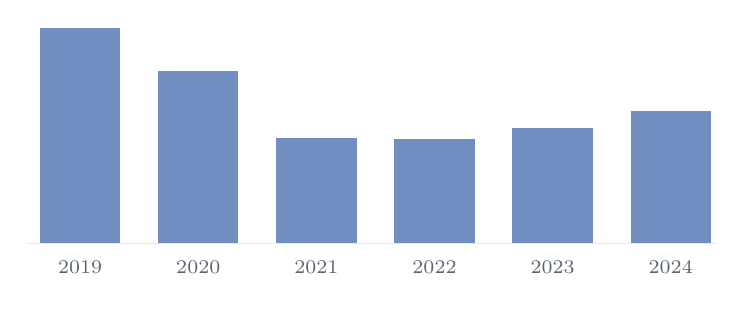
\begin{tikzpicture}[y=0.58mm]
      \foreach \h/\yr [count=\i from 0] in {47.3/2019, 37.8/2020, 23.2/2021,
                                           23.0/2022, 25.3/2023, 29.0/2024} {
        \fill[calm!80] (\i*1.5,0) rectangle ++(1.02,\h);
        \node[below=1mm,font=\scriptsize,text=muted] at (\i*1.5+0.51,0) {\yr};
      }
      \draw[border,line width=0.4pt] (-0.15,0) -- (8.6,0);
    \end{tikzpicture}\\[0.5mm]
    {\scriptsize\color{muted}清洗后各年行数（千），六年合计 185,632 行}
  \end{center}

  \vfill
  {\small 汇报人：曾子睿 \hfill 2026 年 10 月}\\[1mm]
  {\tiny\color{muted}原始数据版权归 JetBrains / PSF 所有，此处只涉及清洗脚本与统计口径。}
\end{frame}

% ---------------------------------------------------------------- 02 关键数字
\begin{frame}{这两周学习了什么}
  \lead{初步学习了数据清洗，把六份原始 CSV 洗成六份能直接读的表}

  \begin{columns}[T,onlytextwidth]
    \column{0.235\textwidth}\kpi{6}{个年份，2019--2024}{calm}
    \column{0.235\textwidth}\kpi{2,408}{原始列（六年合计）}{good}
    \column{0.235\textwidth}\kpi{18,011}{删除的行（8.8\%）}{accent}
    \column{0.235\textwidth}\kpi{2,054}{二值化的多选列}{ink}
  \end{columns}

  \vspace{2.5mm}
  {\small 行数从 203,643 变成 185,632，删掉的都是空行和重复行。}

  \src{来源：\code{cleaned/cleaning\_report.md}}
\end{frame}

% ---------------------------------------------------------------- 03 数据结构
\begin{frame}{先看清数据长什么样}
  \lead{六年列数从 290 涨到 573，其中七成以上是选择题按选项拆出来的列。}

  \begin{center}
    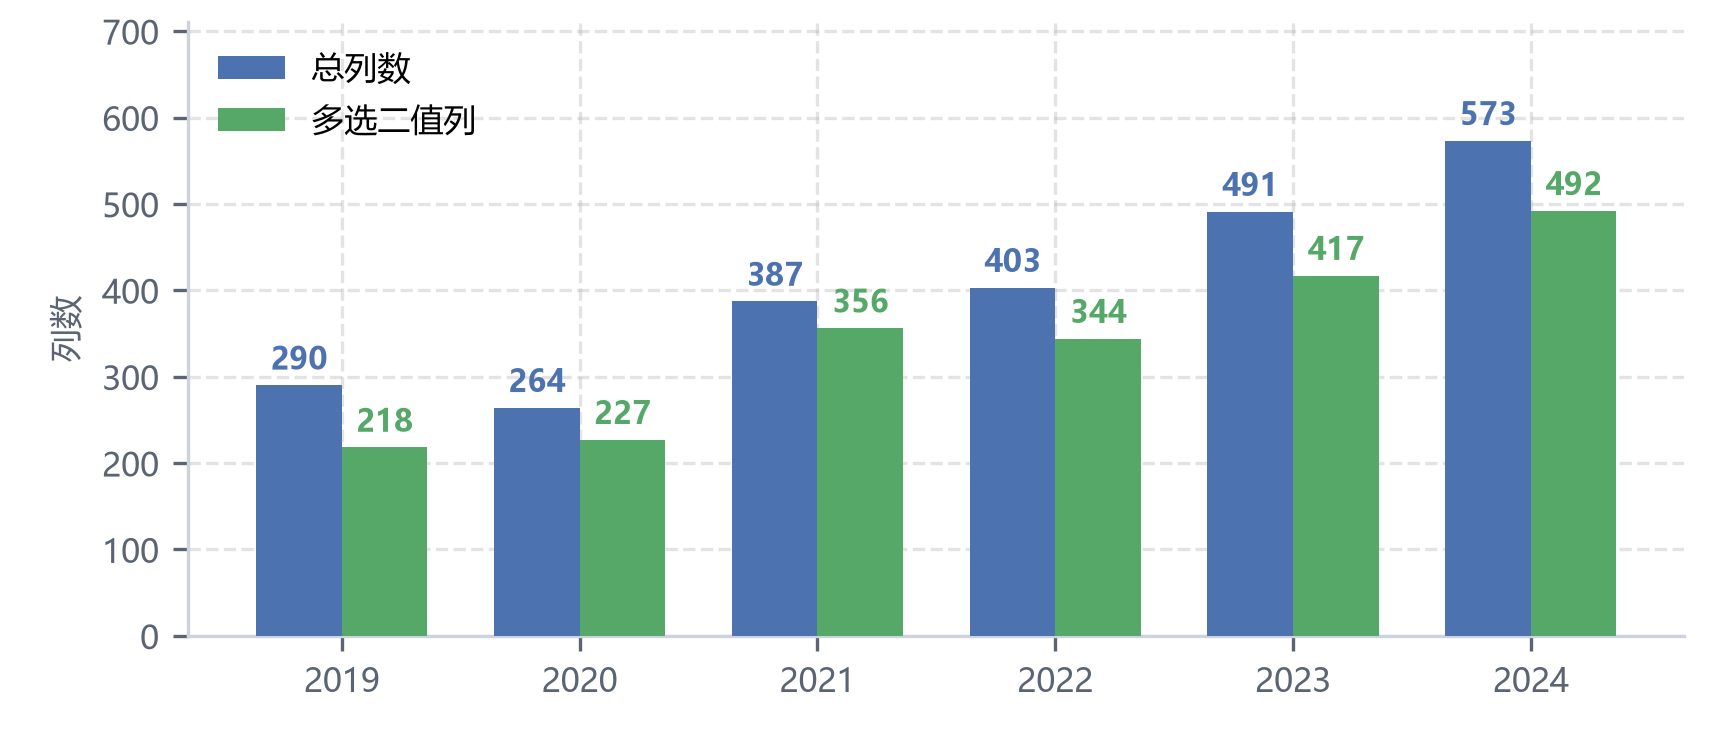
\includegraphics[width=\textwidth,height=0.72\textheight,keepaspectratio]{../figures/f2_structure_growth.png}
  \end{center}

  \src{表头有两套写法：2019 年是整句问句，2020 年以后是点分前缀。}
\end{frame}

% ---------------------------------------------------------------- 04 学习路径
\begin{frame}{两周的学习}
  \lead{从数据本身的问题出发，一个问题一个问题解决。}

  \begin{columns}[T,onlytextwidth]
    \column{0.235\textwidth}\raggedright
      {\color{calm}\bfseries\Large 01}\\[1mm]{\bfseries 认数据}\\[0.6mm]
      {\scriptsize\color{muted}列数在涨吗？}\\[1.6mm]
      {\scriptsize 行列多少，表头有几种，\\缺失到什么程度。\\先看不写。}
    \column{0.235\textwidth}\raggedright
      {\color{calm}\bfseries\Large 02}\\[1mm]{\bfseries 定口径}\\[0.6mm]
      {\scriptsize\color{muted}缺失怎么算？}\\[1.6mm]
      {\scriptsize 没回答、写了 NA、答了 None 是三件事，做好区分。}
    \column{0.235\textwidth}\raggedright
      {\color{accent}\bfseries\Large 03}\\[1mm]{\bfseries 洗单元格}\\[0.6mm]
      {\scriptsize\color{muted}哪些行是废的？}\\[1.6mm]
      {\scriptsize 空白、标点、全角半角，还有整行重复。}
    \column{0.235\textwidth}\raggedright
      {\color{good}\bfseries\Large 04}\\[1mm]{\bfseries 规范列名}\\[0.6mm]
      {\scriptsize\color{muted}说的是同一件事吗？}\\[1.6mm]
      {\scriptsize 问句表头转点分，多选题拆成 0/1 列。}
  \end{columns}

  \vspace{3mm}
  {\small 每问完一步就回数据里数一遍，数不对就说明上一步的口径错了。}

  \src{数据：仓库根目录六份原始 CSV 与 \code{cleaned/} 下的清洗产物}
\end{frame}

% ---------------------------------------------------------------- 05 缺失口径
\begin{frame}{第一课：没回答和答了 None 是两回事}
  \lead{pandas 默认会把 None 读成缺失，可这份数据里 None 是答案。}

  \begin{columns}[T,onlytextwidth]
    \column{0.32\textwidth}\raggedright
      {\bfseries 未回答}\\[1.2mm]
      {\scriptsize 受访者跳过这题，格子里就是空的。不能当 0，也不能当「否」。}
    \column{0.32\textwidth}\raggedright
      {\bfseries N/A 之类的写法}\\[1.2mm]
      {\scriptsize 代码里收了 NA、n/a、nan 等六种写法，统一归成空字符串。}
    \column{0.32\textwidth}\raggedright
      {\bfseries None 是答案}\\[1.2mm]
      {\scriptsize 「一个都不用」是有效信息，必须原样留着。}
  \end{columns}

  \vspace{3mm}
  \begin{tcolorbox}[enhanced,colback=ink,colframe=ink,boxrule=0pt,arc=1mm,
      left=3mm,right=3mm,top=2mm,bottom=2mm]
    {\ttfamily\scriptsize\color{white} pd.read\_csv(path, encoding="utf-8-sig", keep\_default\_na=False)}
  \end{tcolorbox}

  \vspace{2mm}
  {\color{warn}\bfseries 25.5\%}\;\;{\small 2019 年 \code{is.python.main} 的未回答比例。问卷跳答，不能补 0，也不能算作「否」。}

  \src{来源：\code{clean\_survey.py}（\code{MISSING\_TOKENS}）；缺失率由 \code{cleaned\_2019.csv} 实测。}
\end{frame}

% ---------------------------------------------------------------- 06 流水线
\begin{frame}{六步清洗}
  \lead{顺序不能乱，每一步只解决一类问题。}

  \begin{center}
    \begin{tikzpicture}[start chain=going right,node distance=0.5cm,
        st/.style={on chain,draw=border,fill=panel,rounded corners=0.8mm,align=center,
            text width=1.72cm,inner sep=2pt,minimum height=1.5cm,font=\scriptsize},
        every join/.style={->,draw=border,line width=0.9pt}]
      \node[st]{\textbf{01}\\[1mm]缺失归空};
      \node[st,join]{\textbf{02}\\[1mm]列名规范化};
      \node[st,join]{\textbf{03}\\[1mm]去空行空列};
      \node[st,join]{\textbf{04}\\[1mm]去重复行};
      \node[st,join]{\textbf{05}\\[1mm]多选二值化};
      \node[st,join]{\textbf{06}\\[1mm]数值转换};
    \end{tikzpicture}
  \end{center}

  \vspace{3mm}
  \begin{columns}[T,onlytextwidth]
    \column{0.31\textwidth}
      {\bfseries 归空要在改列名之前}\\[1mm]
      {\scriptsize 判重要按内容比，列名一变就对不上。}
    \column{0.31\textwidth}
      {\bfseries 去重要在二值化之前}\\[1mm]
      {\scriptsize 0/1 化会把原本不同的两行洗成一样。}
    \column{0.31\textwidth}
      {\bfseries 列只改不删}\\[1mm]
      {\scriptsize 六年空列、重复列都是 0，问题靠重命名和取值统一解决。}
  \end{columns}

  \src{来源：\code{clean\_survey.py}、\code{cleaned/cleaning\_report.md}}
\end{frame}

% ---------------------------------------------------------------- 07 删行结果
\begin{frame}{删掉的 18,011 行是怎么来的}
  \lead{九成集中在 2020 年，那里混着 12,554 个全空行和 4,115 个重复行。}

  \begin{center}
    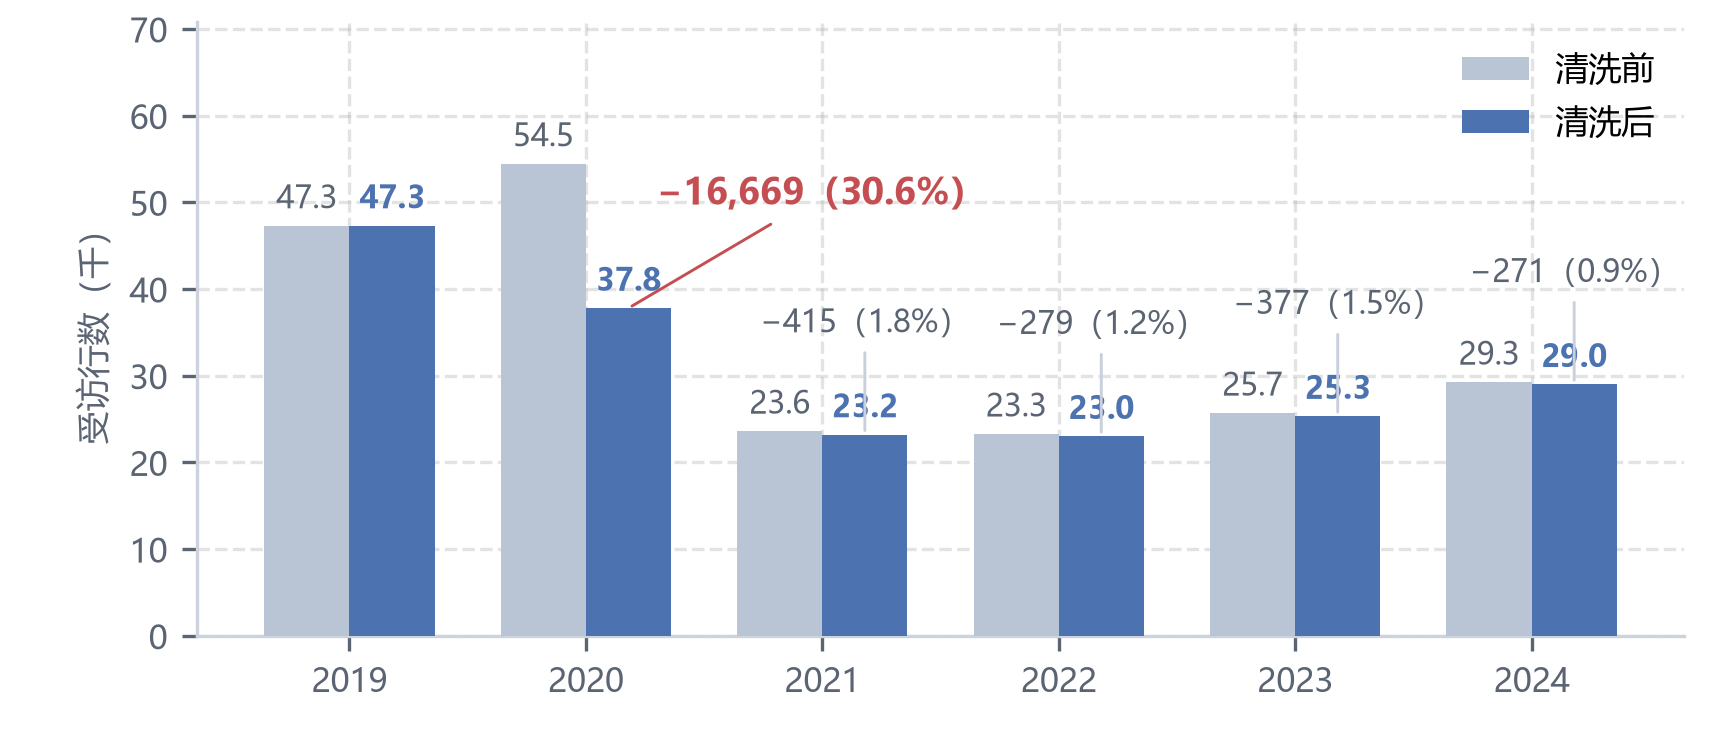
\includegraphics[width=\textwidth,height=0.72\textheight,keepaspectratio]{../figures/f1_rows_before_after.png}
  \end{center}

  \src{其他年份只删重复回答：2021 年 415 行、2022 年 279 行、2023 年 377 行、2024 年 271 行。}
\end{frame}

% ---------------------------------------------------------------- 08 列名规范化
\begin{frame}{列名规范化：问句表头怎么变成点分命名}
  \lead{2019 年的表头是整句问句，选项在冒号前面，得先拆开再套上统一的组前缀。}

  {\scriptsize
    \begin{tabular}{@{}p{6.35cm}p{6.35cm}@{}}
      \toprule
      {\bfseries 2019 原始表头} & {\bfseries 规范化之后} \\
      \midrule
      \code{Is Python the main language\ldots} & \code{is.python.main} \\
      \code{Bash / Shell:What other language\ldots} & \code{other.lang.Bash / Shell} \\
      \code{What do you use Python for?[Data analysis]} & \code{other.purposes.Data analysis} \\
      \bottomrule
    \end{tabular}
  }

  \vspace{2.5mm}
  {\small 2019 年一共改了 289 个列名。重名的两列在旧列名后加 \code{\_\_dup} 后缀，不合并。}

  \vspace{1.5mm}
  {\small 没解决的是组路径：环境隔离 2020 年挂在 \code{isolate.environments}，2023 年挂在 \code{environments.isolate}；后续将研究如何合并。}

  \src{来源：\code{clean\_survey.py}（\code{rename\_columns}）、\code{cleaned/cleaning\_report.md}}
\end{frame}

% ---------------------------------------------------------------- 09 多选二值化
\begin{frame}{多选题：2,054 列改成 0/1}
  \begin{center}
    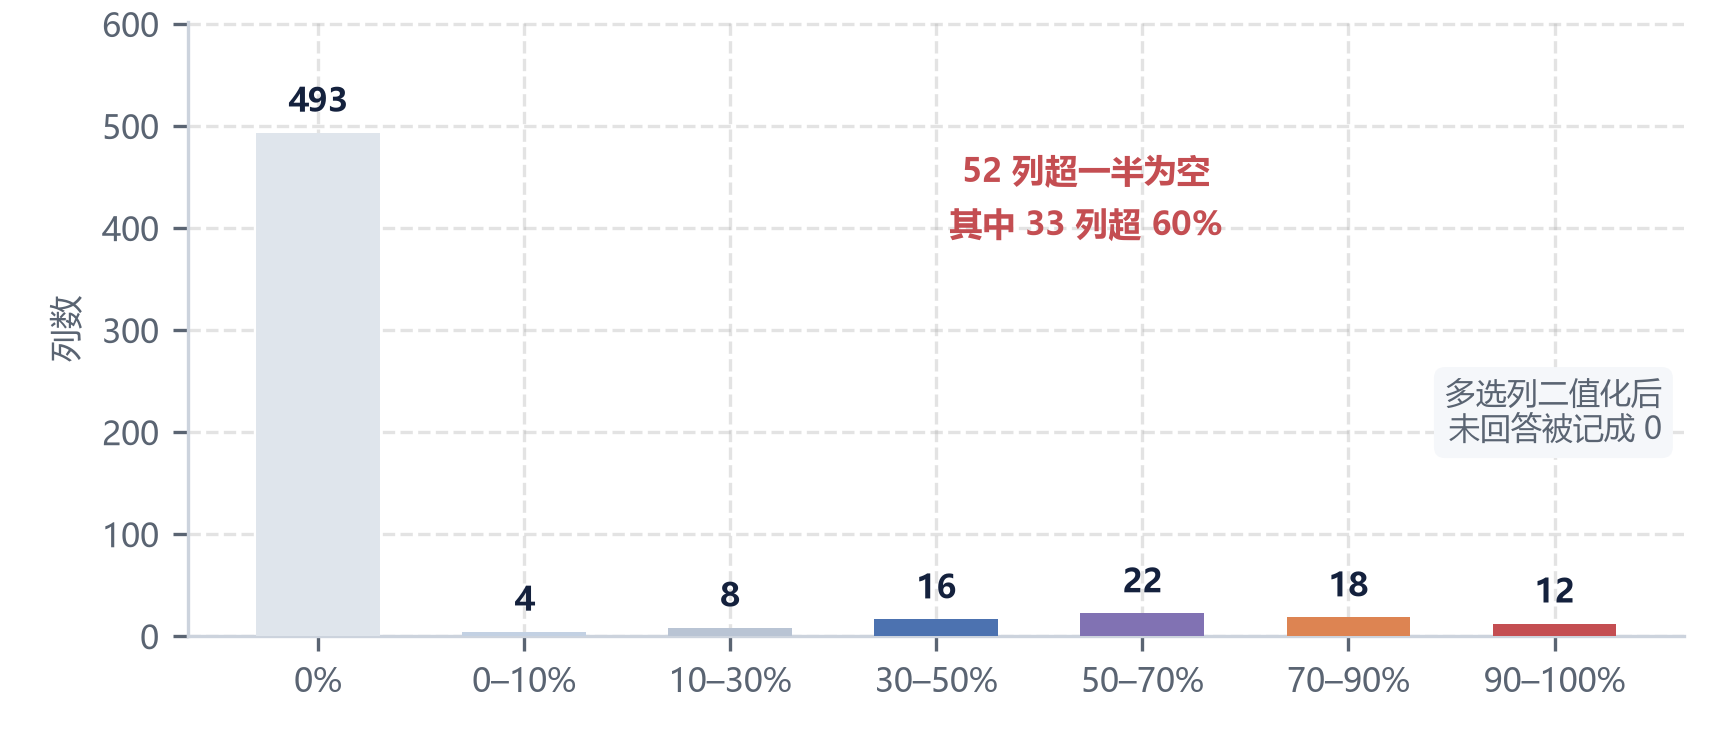
\includegraphics[width=\textwidth,height=0.56\textheight,keepaspectratio]{../figures/f3_missing_profile.png}\\[0.5mm]
    {\scriptsize\color{muted}2024 年 573 个列的缺失率分布：横轴是缺失率区间，纵轴是列数}
  \end{center}

  {\small 代价是：二值化以后，\code{0} 既表示「没勾」，也表示「这题没答」。2024 年 573 列里有 493 列因此看不出缺失。}

  \src{来源：\code{clean\_survey.py}（\code{binarize\_multiselect}）；缺失率由 \code{cleaned\_2024.csv} 实测。}
\end{frame}

% ---------------------------------------------------------------- 10 复盘
\begin{frame}{复盘：学会了什么，还没做什么}
  \lead{清洗这一段算是走通了，但整个流程只完成了开头。}

  \begin{columns}[T,onlytextwidth]
    \column{0.47\textwidth}
      {\bfseries\color{good} 已经做的}\\[2mm]
      {\small
        \begin{itemize}\setlength{\itemsep}{0.8mm}
          \item 口径写在代码里：缺失标记、分母、二值化规则都能查到出处。
          \item 步骤之间有依赖，顺序定下来就不容易错。
          \item 每一步都留了数量，改完能立刻核对有没有洗坏。
        \end{itemize}}
    \column{0.47\textwidth}
      {\bfseries\color{accent} 还没做的}\\[2mm]
      {\small
        \begin{itemize}\setlength{\itemsep}{0.8mm}
          \item 跨年对齐：列名和取值都还没统一，现在只能一年一年看。
          \item 统计与图表：只学了方法，没产出结论。
          \item 口径文档：目前散在脚本注释里，还没整理成一份说明。
        \end{itemize}}
  \end{columns}

  \vspace{2.5mm}
  {\small 下一步先把对齐补上，再谈跨年比较。}

  \src{谢谢大家！}
\end{frame}

\end{document}
